\section{Ottimizzazione DB}

\subsection{Indici}

Un \textbf{indice} in un sistema di gestione di database (DBMS) è una struttura dati organizzata che consente di individuare rapidamente un determinato record all'interno di un file di dati. Uno dei principali vantaggi dell'utilizzo degli indici è il \textbf{miglioramento delle prestazioni delle query}: gli indici permettono di ridurre il tempo necessario per cercare i dati, evitando una scansione completa della tabella.

Creare indici sui campi che vengono frequentemente utilizzati nei filtri delle query (ad esempio, con condizioni \texttt{WHERE}, \texttt{JOIN}, \texttt{ORDER BY} o \texttt{GROUP BY}) può velocizzare significativamente l'elaborazione delle richieste, ottimizzando il sistema nel suo complesso.

Tuttavia, è importante bilanciare l'uso degli indici per evitare costi aggiuntivi durante le operazioni di scrittura come \texttt{INSERT}, \texttt{UPDATE} e \texttt{DELETE}, poiché gli indici devono essere aggiornati ogni volta che i dati della tabella vengono modificati.

Tralasciando gli indici sulla chiave primaria, in quanto il DBMS crea un indice per ogni chiave primaria della tabella, abbiamo ritenuto opportuna l'aggiunta dei seguenti indici: \\

\begin{lstlisting}
-- utile per filtrare missioni sullo stato
CREATE INDEX idx_missioni_stato ON MISSIONI(Stato); 

-- utile per filtrare sul ruolo dei membri
CREATE INDEX idx_membri_ruolo ON MEMBRI(Ruolo); 

-- utile per filtrare sul tipo di robot
CREATE INDEX idx_robot_tipo ON ROBOT(Tipo); 

-- utile per filtrare sulla data del report
CREATE INDEX idx_report_data ON REPORT(Data);

-- utile per filtrare sulla coppia sensore-data di una rilevazione
CREATE INDEX idx_rilevazioni_sensori_data ON RILEVAZIONI(Sensori, Data);
\end{lstlisting}

\subsection{Concorrenza}

Per la gestione della concorrenza, si è scelto di adottare il protocollo \textbf{2PL stretto} (\textit{Strict Two-Phase Locking}), una variante del protocollo \textbf{2PL} (\textit{Two-Phase Locking}). Entrambi i protocolli si basano sul meccanismo dei \textbf{lock}, il quale consente di controllare l'accesso concorrente agli oggetti condivisi e garantisce la \textbf{serializzabilità delle transazioni}, assicurando che il risultato delle operazioni concorrenti sia equivalente a una loro esecuzione sequenziale.
\noindent
\\Il protocollo 2PL stretto segue le seguenti regole operative:


\begin{itemize}
    \item \texttt{lock()}: ogni oggetto coinvolto nelle operazioni è protetto da un lock per controllare l'accesso concorrente.;
    \item \texttt{read\_lock()}: quando una transazione desidera leggere un oggetto, viene applicato un lock di lettura. Questo tipo di lock consente a più transazioni di leggere contemporaneamente lo stesso oggetto, permettendo una condivisione sicura;
    \item \texttt{write\_lock()}: Quando una transazione desidera modificare un oggetto, viene applicato un lock di scrittura. Questo lock è esclusivo, consentendo a una sola transazione per volta di effettuare modifiche sull’oggetto;
    \item \texttt{unlock()}: ogni lock deve essere rilasciato una volta terminata l'operazione corrispondente, consentendo ad altre transazioni di accedere all’oggetto;
\end{itemize}

\noindent
Gli oggetti possono trovarsi in tre stati: \textbf{libero}, \textbf{bloccato in lettura}, o \textbf{bloccato in scrittura}.\\
\noindent \\
La scelta del \textbf{2PL stretto} rispetto al \textbf{2PL} è dovuta al fatto che il \textbf{2PL stretto} evita l'anomalia delle \textbf{letture sporche} (\textit{dirty reads}), che possono verificarsi in altri approcci di gestione della concorrenza.

Il protocollo 2PL stretto (Strict Two-Phase Locking) si articola in due fasi principali, che regolano l'acquisizione e il rilascio dei lock da parte delle transazioni:

\begin{enumerate}
    \item \textbf{Fase crescente}
    \begin{itemize}
        \item In questa fase, la transazione acquisisce tutte le risorse necessarie mediante i comandi \texttt{read\_lock} e \texttt{write\_lock}.
        \item La fase crescente termina quando la transazione ha acquisito tutti i lock necessari per completare le proprie operazioni.
    \end{itemize}
    \item \textbf{Fase decrescente}
    \begin{itemize}
        \item Questa fase inizia quando la transazione rilascia il primo lock mediante il comando \texttt{unlock}.
        \item Nel caso del protocollo \textbf{2PL stretto}, il rilascio dei lock (fase decrescente) può avvenire esclusivamente dopo che la transazione ha eseguito il \textbf{commit} o l'\textbf{abort}, garantendo che le risorse modificate non siano accessibili da altre transazioni fino a quando non sono consolidate o annullate.
    \end{itemize}
\end{enumerate}

Questo approccio garantisce che le transazioni siano serializzabili, impedendo conflitti e mantenendo la consistenza dei dati.

\subsection{Affidabilità}

Il controllo di \textbf{affidabilità} in un sistema di basi di dati ha come obiettivo principale il \textbf{ripristino} dello stato corretto del sistema (recovery) in seguito a guasti accidentali o intenzionali, che possano compromettere la funzionalità del sistema stesso. I guasti possono essere legati sia a malfunzionamenti hardware (ad esempio, guasti su disco o memoria) che software (ad esempio, crash di applicazioni o errori di sistema).

Il sistema di affidabilità si basa sulla gestione delle \textbf{transazioni}, che sono le unità fondamentali delle operazioni nel database, garantendo \textbf{atomicità} (le transazioni sono eseguite in modo completo o non eseguite affatto) e \textbf{persistenza} (i dati delle transazioni devono essere memorizzati in modo permanente una volta che la transazione è stata completata correttamente).

\subsubsection{Backup}

Per garantire un alto livello di affidabilità, il nostro sistema di database implementa la strategia di backup RAID 1, che offre una soluzione di mirroring. In un sistema RAID 1, ogni dato scritto sul disco primario viene duplicato in tempo reale su un disco secondario, chiamato "mirror". Questa tecnica garantisce che, in caso di guasto di uno dei dischi, i dati siano ancora disponibili sull'altro disco, riducendo il rischio di perdita di informazioni e migliorando la disponibilità del sistema.

\begin{figure}[h]
    \centering
    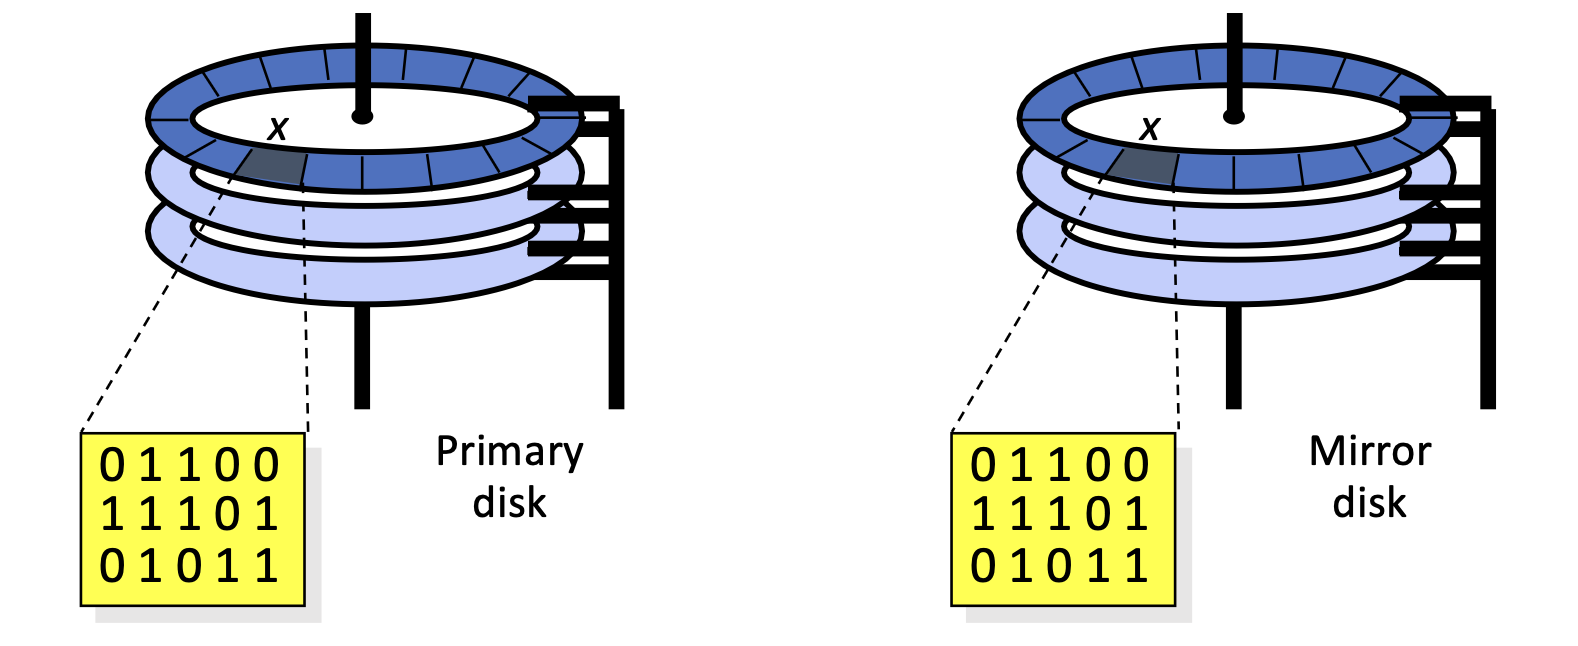
\includegraphics[width=0.5\textwidth]{Media/raid.png}
    \caption{RAID 1 Mirroring}
    \label{fig:raid}
\end{figure}

\subsubsection{Recovery}

Il gestore dell’affidabilità deve gestire l’esecuzione dei comandi transazionali di \texttt{begin transaction}, \texttt{commit}, \texttt{rollback} e tutte le operazioni di ripristino dopo i guasti.

Per poter effettuare ciò, il gestore deve possedere un file di log: un file presente su memoria stabile che registra tutte le operazioni svolte dalle transazioni nel loro ordine di esecuzione.

Il log è quindi una sorta di “diario di bordo” che, in un qualsiasi istante, permette di ricostituire il contenuto corretto della base dei dati a seguito di malfunzionamenti.

\begin{figure}[h]
    \centering
    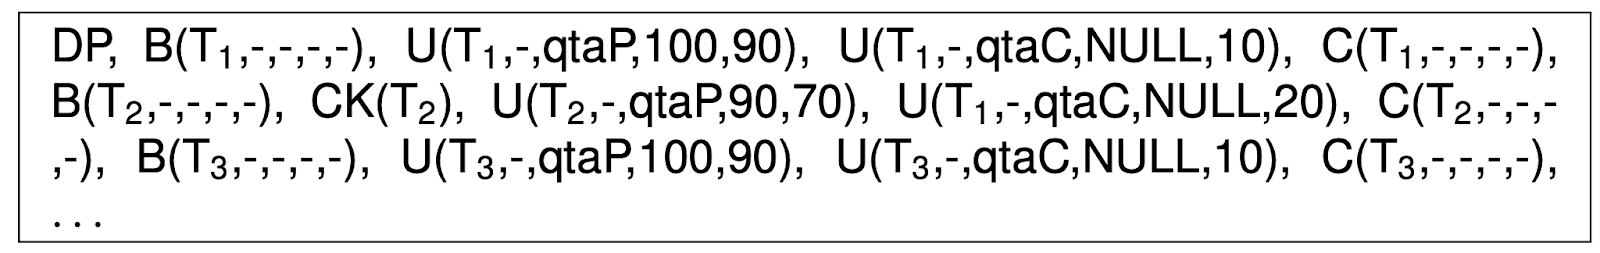
\includegraphics[width=0.8\textwidth]{Media/log.png}
    \caption{File di log}
    \label{fig:log}
\end{figure}

\paragraph{Tecniche di recovery}

\begin{itemize}
    \item \textbf{Ripresa a freddo}:  
    In caso di guasti hardware che interessano i dispositivi di memoria di massa (ad esempio, guasti ai dischi rigidi), si verifica la perdita del contenuto sia della memoria centrale che di quella secondaria. Tuttavia, la memoria stabile, come i dispositivi di backup, rimane intatta. In tali circostanze, si procede con una \textbf{ripresa a freddo} (\emph{cold restart}), che comporta un ripristino approfondito. Questo processo richiede il recupero dei dati mediante l'uso di backup e log disponibili.
    \item \textbf{Ripresa a caldo}:  
    Nei casi di guasti software (come errori di programma, crash di sistema, interruzioni dell’alimentazione, ecc.), viene compromesso esclusivamente il contenuto della memoria centrale, mentre la memoria secondaria e quella stabile rimangono intatte. In queste situazioni si procede con la \textbf{ripresa a caldo} (\emph{warm restart}), che consente un ripristino più rapido rispetto alla ripresa a freddo.
\end{itemize}

Indipendentemente dal tipo di ripresa adottata, la procedura di recovery segue tre fasi principali, secondo il \textbf{Modello Fail-Stop}:

\begin{enumerate}
    \item \textbf{Arresto delle transazioni attive}:  
    Tutte le transazioni attualmente in esecuzione sul sistema di basi di dati vengono forzatamente interrotte per evitare ulteriori inconsistenze.
    
    \item \textbf{Ripristino del sistema operativo}:  
    Si procede al riavvio e alla verifica del corretto funzionamento del sistema operativo, necessario per garantire l’esecuzione della fase successiva.
    
    \item \textbf{Esecuzione del ripristino}:  
    Viene avviata la procedura di recupero, che sfrutta backup, log e informazioni residue per ripristinare la consistenza e l'integrità del database.
\end{enumerate}

Queste tecniche, basate sul modello \textbf{fail-stop}, mirano a garantire la continuità operativa e la salvaguardia dei dati, anche in presenza di guasti critici.
